\documentclass[preprint,5p,times]{elsarticle}

%%%%%%%%%%%%%%   Preample  %%%%%%%%%%%%%%%%%%
%% for comment (texts in between \begin{comment} and \end{comment} will be ignored)
\usepackage{comment} 

%% The amssymb package provides various useful mathematical symbols
\usepackage{amssymb}
%% The amsthm package provides extended theorem environments
\usepackage{amsthm}

%% for celcius symbol
\usepackage{textcomp}

%% for units
\usepackage{siunitx}

%% multirow
\usepackage{multirow}

%% The lineno packages adds line numbers. Start line numbering with
%% \begin{linenumbers}, end it with \end{linenumbers}. Or switch it on
%% for the whole article with \linenumbers.
\usepackage{lineno}
\linenumbers

%% package for subfigure environment
\usepackage{subcaption}

%% package for type Greek letters without entering into math-mode
\usepackage{textgreek}

%% package for large picture in two-colume
%\usepackage{dblfloatfix}
%\usepackage{fixltx2e}

%% only jpg pdf eps are allowed,tiff format are not allowed in latex
%% eps in principle can't be compiled by pdflatex,pdf not compiled by latex,but Kile can do some intermedate conversion to allow this happen.
\DeclareGraphicsExtensions{.pdf,.eps,.jpg}
%%opening
\journal{NIMA}

\begin{document}

%%%%%%%%%%%%%% Front Matter %%%%%%%%%%%%%%%%%%
\begin{frontmatter}

\title{A versatile PMT test bench and the measurements of 500 Hamamastu R4443-Mod2 phototubes for DAMPE-PSD detector}
%%\title{Title with footnote\tnoteref{t1}}
%%\tnotetext[t1]{FootNote for title}

\author[imp,ucas,lzu]{Yong Zhou}
%\ead{yong@impcas.ac.cn}

\author[imp]{Yuhong Yu}
%%\ead{yuyuhong@impcas.ac.cn}

\author[imp]{Zhiyu Sun\corref{corresponding_author}}
\cortext[corresponding_author]{Corresponding author}
\ead{sunzhy@impcas.ac.cn}

%% Additional Author information %%
%%\author[ano]{Anonymous\fnref{fn1}}
%%\ead{anonymous@anonymous.cn}
%%\fntext[fn1]{FootNote for Anonymous author}

\address[imp]{Institute of Modern Physicas,Chinese Academy of Sciences, 509 Nanchang Road, Lanzhou, 730000, P.R.China}
\address[ucas]{Graduate University of the Chinese Academy of Sciences, 19A Yuquan Road, Beijing, 100049, P.R.China}
\address[lzu]{School of Nuclear Science and Technology, Lanzhou University, 222 South Tianshui Road, Lanzhou, 730000, P.R.China}
%%\address[ano]{Anonymous Address of Anonymous author}

%%
\begin{abstract}
blablabla
\end{abstract}

%%
\begin{keyword}
keyword1
\sep keyword2
\sep keyword3

%% PACS codes here, in the form: \PACS code \sep codes

%% MSC codes here, in the form: \MSC code \sep code
%% or \MSC[2008] code \sep code (2000 is the default)

\end{keyword}

\end{frontmatter}

%%%%%%%%%%%%%%%%  Introduction  %%%%%%%%%%%%%%%%%%%%%%%
\section{Introduction}
\label{sec:introduction}

DArk Matter Paricle Explorer(DAMPE)\cite{Chang_Jin_dampe} is a satellite-borne particle detector for dark matter search and cosmic ray study.
It is designed to cover the energy range from 5~GeV to 10~TeV for electrons and photons with an energy resolution of 1\% at 800~GeV,from 100~GeV to 1~PeV for heavy ions with an energy resolution better than 40\% at 800~GeV.

Plastic scintillator Strip Detector(PSD),which sits at the topmost of the satellite,is a key component of DAMPE detector.
By measuring the energy deposit of particles pentrating through it,PSD serves as a anti-coincidence detector for e/$\gamma$ discrimination as well as a detector for charge measurement up to Z=20.
PSD consists of 82 plastic scintillator strips(EJ-200\cite{ej200}) of dimention $864mm\times28mm\times10mm$,each readout at both ends by a Hamamastu R4443-Mod2 photomultiplier tube.
These strips are arranged into two orthogonally oriented layers,convering an effective area of $820mm\times820mm$.
Each PMT is readout at both dynode 5 and dynode 8 with different gains to cover the large dynamic range from $\sim$0.5~MIPs to $\sim$700~MIPs.
The readout signals are processed by a highly-sensitive ASIC chip(VA32) with the range of 0-14~pC,and then digitized by an ADC with 14~bits resolution.

Unlike groud-based experiments,the power supply system of DAMPE payload can only provide discrete high voltage levels with an interval of 30~V.
Furthermore,every 6 or 7 PMTs of PSD form a HV-group and share the same high voltage channel.
In this case,the ususal method of fine-tuning individual PMT's high voltage to get optimal gain is not available.  
The characteristics of PMTs in the same HV-group should have similar dependency on voltage.
Thus a careful selection of the tubes is mandatory to get uniform energy response across the whole detector and optimal utilization of the mesuring range.
For this selection,the gain of dynode 5 and dynode 8 as a function of supplying voltage needs to be measured precisely.  

On the other hand,the harsh environment of satellite imposes a strict set of quality control processes for the production of PMT modules,as shown in Fig.~\ref{fig:production_procedure}.
A PMT module is composed of a bare PMT tube,a layer of permalloy for magnetic shielding,baseboards for HV divider and signal readout,silicone rubber for coupling with the palstic scintillator,pouring sealant to protect PMT from vibration and HV breakdown and the supporting Aluminum box.
\begin{figure}[h!]
 \centering
 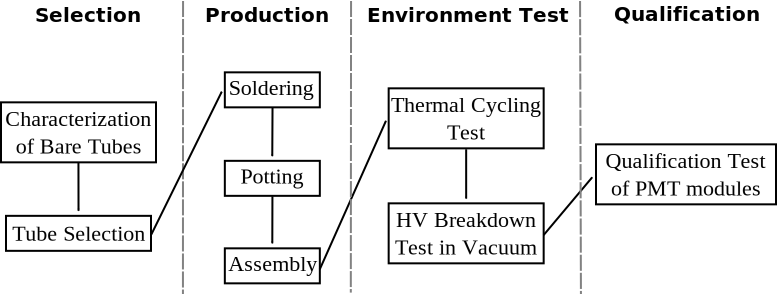
\includegraphics[width=90mm]{pmt_production_procedure}
\caption{Production Procedures of a PMT module.The PMT should be tested during the selection phase and qualification phase}
\label{fig:production_procedure}
\end{figure} 
Some of the PMT modules may get irreversible deterioration,even damage,during these processes.
Thus a qualification test shall be performed to certificate the performance of each PMT module before final installation. 

Considering the large number of tubes involved in the Selection phase and Qualification phase,a PMT test bench for bulk testing was designed and contructed to facilitate this work.
500 bare R4443-Mod2 tubes were thoroughly tested and 200 of them were selected for production and qualification.
Finally,164 PMT modules with the optimal characteristics were installed.
While mainly developped for the DAMPE-PSD project,this test bench has been designed to be as versatile as possible and can be upgaded seamlessly for future experiments.
The detailed description of the test bench will be given in Sec.\ref{sec:description}.Some key characteristics of the test bench is summarized in Sec.\ref{sec:char_testbench}.
The testing results of PSD PMTs and the corresponding selection procedure will be discussed in Sec.\ref{sec:pmt_test}.

%%%%%%%%%%%%%%%% Main Text Body %%%%%%%%%%%%%%%%%%%%%%%
\section{Description of the test bench}
\label{sec:description}

The major design considerations of the test bench are summarized as follows:
\begin{itemize}
 \item \textit{Large capacity}: This is the primary driving force for developping the test bench as indicated in Sec.\ref{sec:introduction}.
 Testing multiple PMTs simultaneously can increase the efficiency and save project time tremendously. 
 \item \textit{Automation}: A single test run ususally takes several hours,during which most operations are trivial jobs like change voltage value,change light intensity,start/stop DAQ,and so on.
 Manual operations are sometimes unreliable in such a long time testing period.
 Thus computer controllable hardwares should be used wherever possible and corresponding software should be developped to automate these trivial operations.
 Manual intervention is only needed in the beginning when mounting PMTs and configuring the testing software and in the end when unmounting PMTs and assessing testing result. 
 \item \textit{Versatility}: The test bench is not designed for single use.
 After its initial use in DAMPE PSD,it will be used for other experiments with different testing requirements.
 Thus potential use cases should be considered and appropriate hardwares should be set up in the first place.
 In particular,moving ability is desirable for characterization of large area PMTs. 
 \item \textit{Flexibility}: As a by product of versatiltiy,flexibility is needed both in terms of hardware and software.
 The hardware platform should be extensible and allow complex testing configurations.
 The software should accommodate any changes in the hardware easily,while keeping the high level functionality unchanged and portable. 
\end{itemize}

A schematic diagram of the final design is shown in Fig.\ref{fig:testbench_overveiw}.
\begin{figure*}[hb]
 \centering
 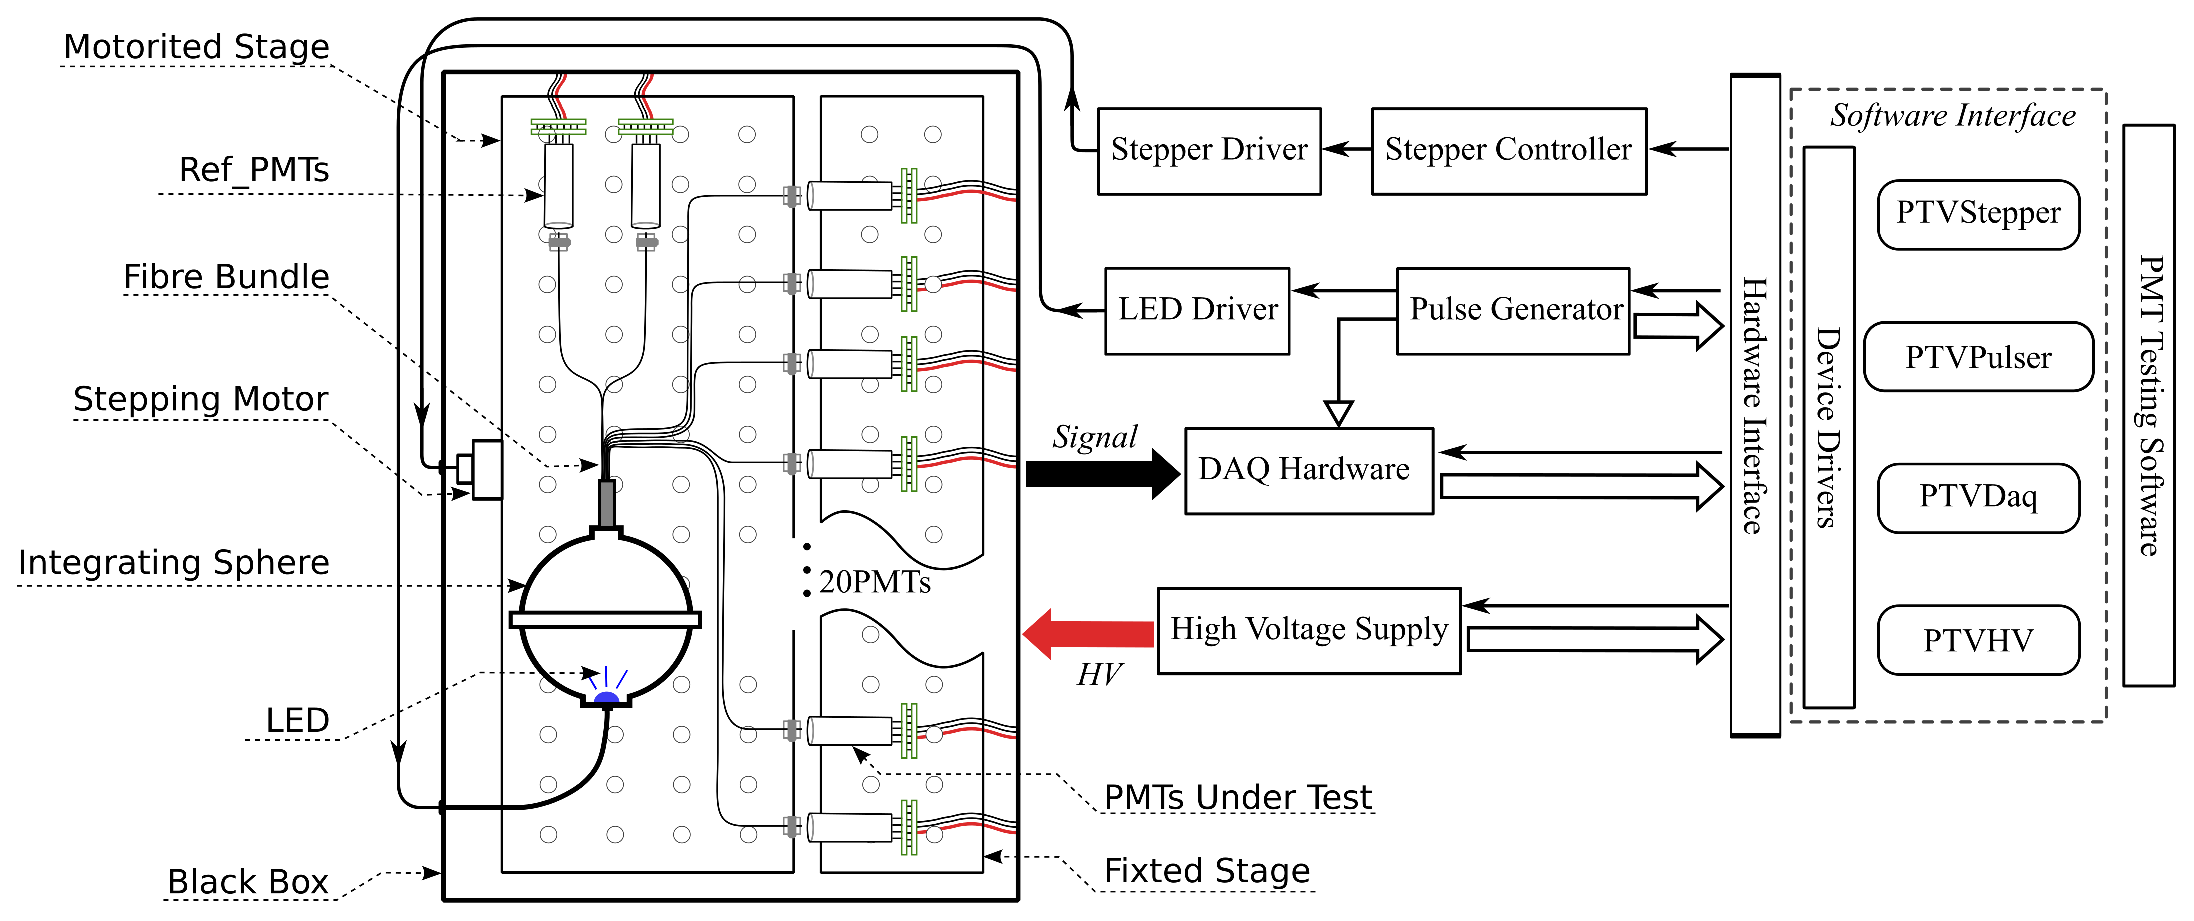
\includegraphics[width=140mm]{testbench_overview}
\caption{Schematic diagram of the PMT test bench system.\textit{PTVStepper},\textit{PTVPulser},\textit{PTVDaq} and \textit{PTVHV} are abstract classes which separate the testing software from the hardware implementation details.}
\label{fig:testbench_overveiw}
\end{figure*}
The test bench is designed to test up to 25 R4443-Mod2 tubes in a single run.
Light flashes from a LED are distributed to each tube's surface through an integrating sphere and a fibre bundle.
Tubes under test,including their bases,are mounted on a fixed stage,while the light source and its distribution system are mounted on a separate three-dimention motorized stage.
This allows scanning of the whole surface of all tested tubes.
Two additional PMTs are mounted in the corner of the motorized stage.
They will not be removed from their fixed positions during all test runs and thus are used as references to monitor the stability of the light source as well as the performance of the whole system.
Both stages are housed in a large light-tight box made of aluminium alloy,with the dimension of $176cm\times100cm\times78cm$.
The box is painted black inside and out and can be opened from the top plate for PMT mounting.
All other devices are located outside the light-tight box.
Cables are led out through various light-tight cable feedthroughs left in the side-plate of the box.
The test bench is sitted in a cleanroom of class 100000,the temperature of which is controlled around 22\textpm2\textcelsius~during test time.

In the following,each key component will be described in detail.
\subsection{Light Source and Distribution}
\label{sec:light_source}

A high-power blue LED(\SI{3}{\watt},\SIrange{465}{485}{\nano\meter}, from Z-light\cite{zlight}) is apdopted as the light source for the test bench.
This product has been used before in the monitoring and calibration system of Neutron Wall Detector at IMP,CAS\cite{yuyuhong_led}. 
A \SI{5}{\centi\meter} diameter integrating sphere is used to convert the LED into a uniform light source.
The integrating sphere is coated interiorly with highly reflective material($\approx$\SI{98}{\percent} at \SI{400}{\nano\meter}) and has two ports of \SI{14}{\milli\meter} diameter.
To get better heat dissipation,the LED is fixed on a special designed base using thermally conductive silicone rubber.
The base is then coupled to the input port of integrating sphere,making the whole sphere as the LED's heat sink.

A bundle of 35 plastic clad silica(PCS) fibres is utilized to distribute light to each PMT under test.
The fibres are \SI{1.5}{\meter} long and have a \SI{400}{\micro\meter} diameter core,a \SI{550}{\micro\meter} diameter cladding.The numerical aperture(NA) is 0.37.
The relatively large core and large NA make the fibre an efficient light extracter of integrating sphere output. 
The input end of the fibre bundle is coupled to the centre of the output port of integrating sphere using a three-dimensional fibre alignment stage.
On the other end,each fibre is fixed using a special designed fibre holder which allows rough position adjustment individually.
Before testing,all used fibres are aligned to the centre of their corresponding PMT's input window with a precision of \SI{0.5}{\milli\meter}.  
For easier manipulation and to protect the fibres from mechanical stress,both ends of the fibre bundle are coated with customized stainless steel ferrules.

An off the shelf hardware,Tektronix AFG3252 arbitrary/function generator,is adpoted as the LED driver.
As a commertial product,various interfaces for remote control are provided in AFG3252,making it suitable for automation.
All of the pulse parameters of AFG3252 can be adjusted in a wide range with high precison,as show in Table \ref{tab:afg3252}.
This is a critical feature for the PMT test of DAMPE PSD,as light intensities covering a large dynamic range are needed to measure the gain ratio between dynode 8 and dynode 5 at different voltages.
\begin{table}[h!]
\caption{Summary of AFG3252 Pulse Mode Characteristics}
\label{tab:afg3252}
 \begin{center}
 \begin{tabular}{lr}
 \multicolumn{2}{l}{Summary of AFG3252 pulse mode characteristics}\\ \hline
 Frequecny & up to \SI{120}{\MHz} \\
 Amplitude & max \SI{5}{\volt} \\
 Pulse width & min \SI{4}{\nano\second} \\
             & resolution \SI{10}{\pico\second} \\
 Leading edge & \SI{2.5}{\nano\second} to 0.625*pusle period \\
 Trailing edge & \SI{2.5}{\nano\second} to 0.625*pusle period \\
 Jitter(typical) & \SI{100}{\pico\second} \\
 Interface     & GPIB,LAN,USB
 \end{tabular}
 \end{center}
\end{table} 
AFG3252 has two independent analog outputs which can be synchronized together.
Thus one of the outputs can be connected to the LED directly,while the other one can generate trigger signal to DAQ. 
Although not designed to be a dedicated LED driver,the stability of AFG3252 is quite satifactory,see Sec.\ref{sec:longterm_stability}.
One limitation of AFG3252 as a LED driver is that it has a limited leading edge of \SI{2.5}{ns}.
This makes it not suitable for timing-related characterizations,where ultra-short(down to hundreds of \si{\pico\second} magnitude) light pulse is needed
In this casse,a dedicated LED driver of special design(commertial or home-made)may be used instead.
But AFG3252 can still be used as a trigger generator to control both the LED driver and DAQ.

\subsection{Three-dimention motorized stage}
\label{sec:platform}

A 3~dimention movable platform was built as the supporting structure

optical breadboard made of stainless steel $156cm\times25cm\times2.5cm$
\subsection{Electronics}
\label{sec:integrating_sphere}

\subsection{High Voltage Supply}
\label{sec:ref_pmt}

\subsection{Software}
\label{sec:software}
The software is developped under Windows and written in C++,which is an efficient language and well suited to the modular design of the test bench.
To facilitate maintainence and future upgrade,the software components are groupped into three hierarchies as following:
\begin{enumerate}
 \item Device abstraction,which not only serves as an interface to the underlying hardwares,but also handles the abstraction of different types of devices. 
 \item Framework libraries,which defines a general testing procedure and provides utility classes for configuration and management.
 \item User inerface,which provides command line based or graphical executables for user interaction. 
\end{enumerate}

Designed as a versatile equipment,different hardware modules may be used in the future.
For example,while the general-purpose VME or CAMAC platform may meet the demands of most of the use cases,some experiments may prefer to use project-specific DAQ hardware for testing.
In another case,a laser light source with a ultra-short pulsing driver may be used for time-related characterization.
Instead of developping a dedicated program each time a hardware interface changes,an abstraction of the devices is adoptted to separate the testing procedure from hardware implementation details.
Abstract classes are defined for four frequently-used devices in PMT testing,i.e. stepper controller,light pulser,DAQ system and HV supplier,as shown in rounded boxes in Fig.\ref{fig:testbench_overveiw}.
Common operations of each type of device are extracted and encapsulated in the corresponding abstract class,which are the only interface to higher level software components.
Concrete classes inheritted from the same abstract class represent different devices of the same type.
Currently,device classes for Leetro MPC07SP motion controller,Tektronix AFG3252 pulse generator,CAEN SY1527 power supply system and DAMPE gound test DAQ board are implemented.
DAQ device class for the CAMAC system based on CC-USB controller is also implemented and thoroughly tested.

Built upon the abstract device inerface,a general testing framework is defined,as shown in Fig.\ref{fig:software_framework}.
As a first step,all used concrete device classes are registered in the singlton class \textit{PTDeviceManager}.
Devices will then be retrieved from \textit{PTDeviceManager} during test.
\begin{figure}[h!]
\centering
 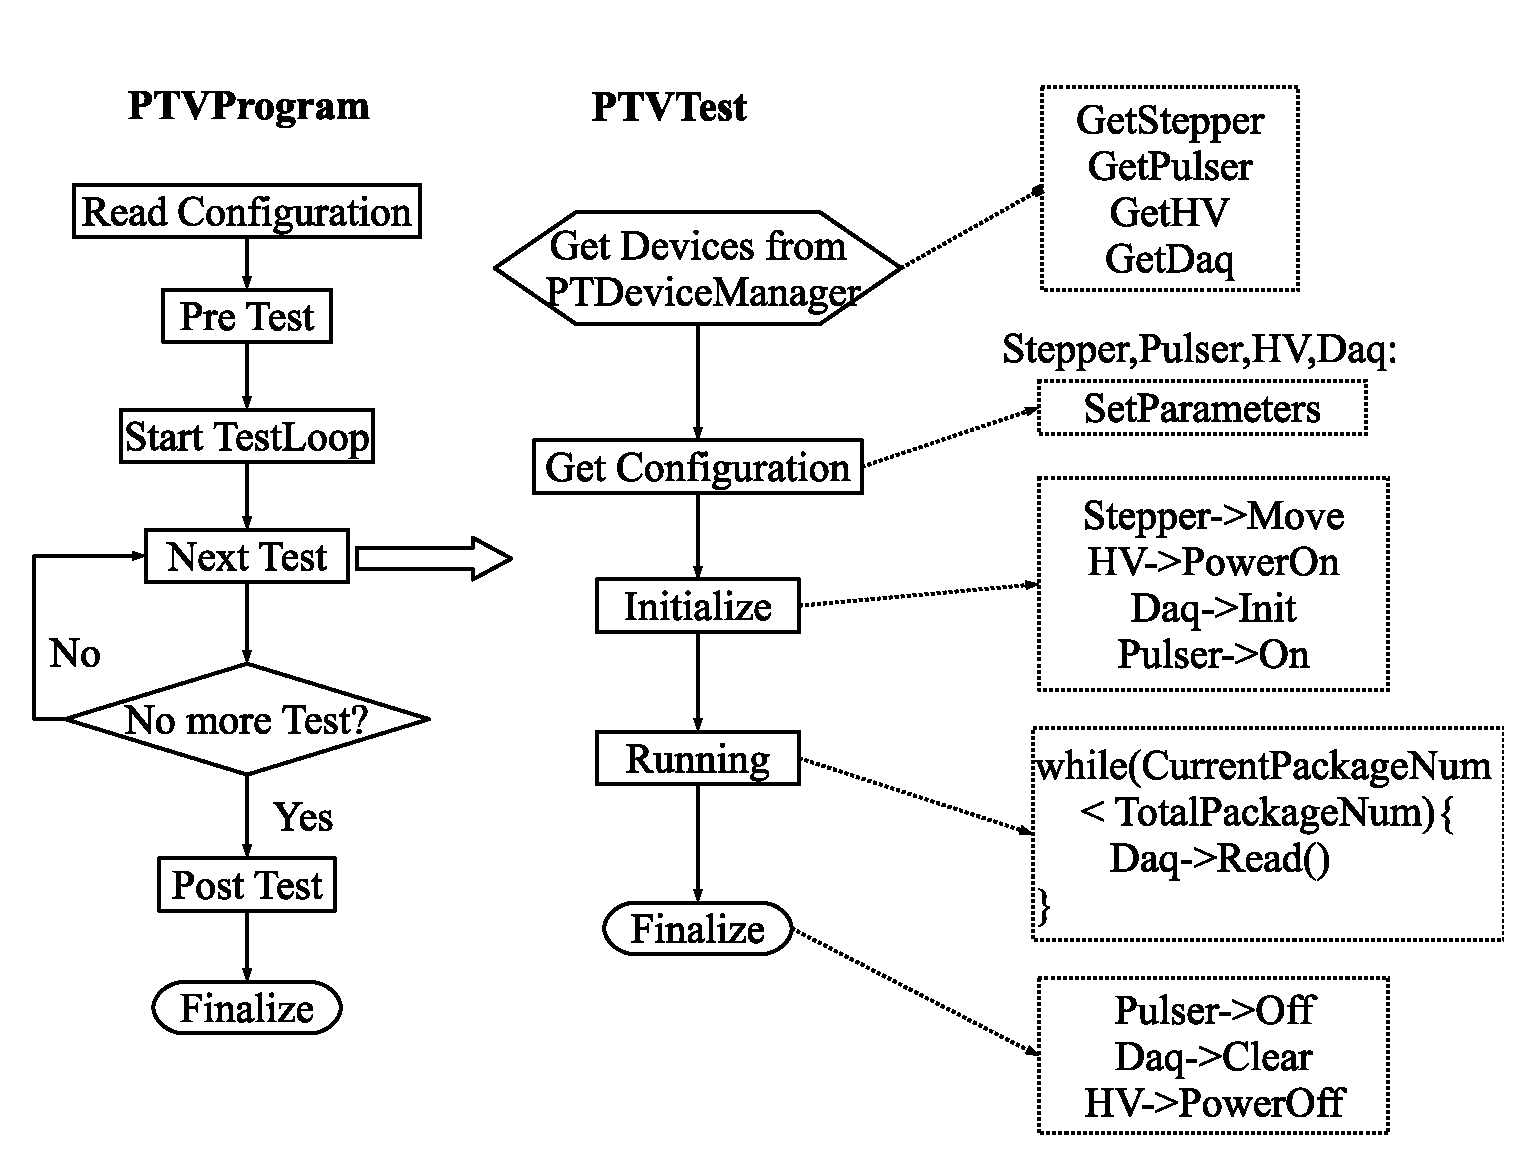
\includegraphics[width=90mm]{software_framework}
\caption{Software framework}
\label{fig:software_framework}
\end{figure}
A \textit{PTVProgram} represents the measurement procedure for a specific characteristic of PMT,such as cathode uniformity,gain,dark count rate,and so on.
\textit{PTVTest} is a subunit of \textit{PTVProgram},which encapsulates the real testing operations performed under a specific condition.
A typical implementation for \textit{PTVTest} using fake code is presented in the third column of Fig.\ref{fig:software_framework}.
Usually,a \textit{PTVProgram} consists of a series of \textit{PTVTest}s,which are invoked sequentially in a test loop.
For example,for cathode uniformity test,the stepping motor will move to a series of positions and the PMT response will be recorded by the DAQ system at each position.
Here,device operations performed at each position constitute a \textit{PTVTest} and tests at all positions constitute a \textit{PTVProgram}.
Additional actions may be added in the \textit{PreTest} method and \textit{PostTest} method of \textit{PTVProgram},which will be invoked before and after the test loop repectively.
Typically,PMT warming shall be performed in \textit{PreTest} and analysis code shall be added in \textit{PostTest}.
\textit{PTVProgram}s of different testing objectives will finally be chained together to constitute a complete characterization of PMT.
Two concrete \textit{PTVProgram}s have been implemented for DAMPE-PSD PMT test.
One for pedestal testing and one for amplitude scan and voltage scan.

Based on the framework library,a light-weight user interface based on PDCurses\cite{pdcurses} has been developped.
This program also incorporates status monitoring function,which is developped utilizing Phtread-win32 library\cite{pthread_win32}.

A dedicated analysis program based on ROOT libraries is also developped for the DAMPE PSD project.
The program does not depends on the framework libraries described above.
The analysis results are inserted into a database for easy query.
\section{Characteristics of the test bench}
\label{sec:char_testbench}

\subsection{Long-term Stability}
\label{sec:longterm_stability}

\subsection{Spatial Uniformity of Integrating Sphere}
\label{sec:spatialuniformity_insph}

\subsection{Transmission Uniformity of Fibre-bundle}
\label{sec:transuniformity_fibre}

\section{PMT testing for PSD}
\label{sec:pmt_test}

\subsection{Selection criteria}
\label{sec:selection}

\subsection{Testing Result of Relative Gain}
\label{sec:relative_gain}

\subsection{Testing Result of Dynode Ratio}
\label{sec:dynode_ratio}

\subsection{PMT Qualification}
\label{sec:qualification}

%%%%%%%%%%%%%%%%  Conclustion   %%%%%%%%%%%%%%%%%%%%%%%
\section{Conclusions}
\label{sec:conclustions}

%%%%%%%%%%%%%%%% Acknowledgement %%%%%%%%%%%%%%%%%%%%%%%
\section*{Acknowledgement}

%%%%%%%%%%%%%%%%    Appendix     %%%%%%%%%%%%%%%%%%%%%%%
%% The Appendices part is started with the command \appendix;
%% appendix sections are then done as normal sections
\appendix
\section{}
\label{app:}

%%%%%%%%%%%%%%%%   Bibliography  %%%%%%%%%%%%%%%%%%%%%%%
%% bibliography style
\section*{References}
\bibliographystyle{elsarticle-num}

%% From BibTex file
\bibliography{mybib}

%% From hand-writing
\begin{comment}
%%\begin{thebibliography}{00}

%%\bibitem{CEBAF12}
%%V.D. Burkert, \emph{arXiv:1203.2373v1 [nucl-ex]}, 2012.

%%\bibitem{CLAS}
%%B.A. Mecking \emph{et al.}, Nucl. Ins. and Meth. in Phys. Research {\bf A503} (2003) 513

%%\end{thebibliography}
\end{comment}

\end{document}
\endinput